\documentclass[10pt]{article}
\usepackage[usenames]{color} %used for font color
\usepackage{amssymb} %maths
\usepackage{amsmath} %maths
\usepackage[utf8]{inputenc} %useful to type directly diacritic characters
\usepackage[letterpaper, portrait, margin=1.5in]{geometry}
\usepackage{graphicx,wrapfig}
\begin{document}
\subsection*{MSDS650 Week 3 Normality Assignment - Nathan Worsham}
Load libraries:
\begin{verbatim}
library(ggplot2)
library(reshape2)
\end{verbatim}
Whenever in code you find yourself repeating the same steps, then either a loop or function should be created. In this case the author creates a function called \verb|assign_vector|. The function performs or replicates the Shapiro-Wilk test on the data provided \textit{n} number of times at 3 different sample sizes--5,10,and 1,000. If \verb|n| is not provided the function defaults to a 1,000 times. Finally the data is made into a data frame, formatted and ordered for the next step. 
\begin{verbatim}
#' @name assign_vector
#' @param data A vector of data to perform the t-test on.
#' @param n An integer indicating the number of t-tests to perform. Default 
   is 1000
#' @return A data frame in "tall" format
assign_vector <- function(data, n = 1000) {
  # replicate the call to shapiro.test n times to build up a vector of p-values
  p.5 <- replicate(n=n, expr=shapiro.test(sample(my.data, 5, replace=
  TRUE))$p.value)
  p.10 <- replicate(n=n, expr=shapiro.test(sample(my.data, 10, replace=
  TRUE))$p.value)
  p.1000 <- replicate(n=n, expr=shapiro.test(sample(my.data, 1000, replace
  =TRUE))$p.value)
  #' Combine the data into a data frame, 
  #' one column for each number of samples tested.
  p.df <- cbind(p.5, p.10, p.1000)
  p.df <- as.data.frame(p.df)
  colnames(p.df) <- c("5 samples","10 samples","1000 samples")
  #' Put the data in "tall" format, one column for number of samples
  #' and one column for the p-value.
  p.df.m <- melt(p.df)
  #' Make sure the levels are sorted correctly.
  p.df.m <- transform(p.df.m, variable = factor(variable, levels = c("5 samples"
            t,"10 samples","1000 samples")))
  return(p.df.m)  
}
\end{verbatim}
After looking over the function and seeing what it returns (on the next step) I found there exists a typo in the function. They call the variable \verb|my.data| but the function calls it \verb|data|, so the function should be this:
\begin{verbatim}
assign_vector <- function(data, n = 1000) {
  p.5 <- replicate(n=n, expr=shapiro.test(sample(data, 5, replace=TRUE))
  $p.value)
  p.10 <- replicate(n=n, expr=shapiro.test(sample(data, 10, replace=TRUE))
  $p.value)
  p.1000 <- replicate(n=n, expr=shapiro.test(sample(data, 1000, replace=
  TRUE))$p.value)
  p.df <- cbind(p.5, p.10, p.1000)
  p.df <- as.data.frame(p.df)
  colnames(p.df) <- c("5 samples","10 samples","1000 samples")
  p.df.m <- melt(p.df)
  p.df.m <- transform(p.df.m, variable = factor(variable, levels = c("5 samples"
  ,"10 samples","1000 samples")))
  return(p.df.m)  
}
\end{verbatim}
Now the test is run with sample data. The data is created using the \verb|rnorm| command which is a "random generation" for the normal distribution, in this case 100,000 random observations. Then the data is run through the function created previously 
\begin{verbatim}
> n.rand <- 100000
> n.test <- 10000
> my.data <- rnorm(n.rand)
> p.df.m <- assign_vector(my.data, n = n.test)
No id variables; using all as measure variables
> head(p.df.m)
   variable     value
1 5 samples 0.6326340
2 5 samples 0.6946454
3 5 samples 0.6202242
4 5 samples 0.9574261
5 5 samples 0.3541403
6 5 samples 0.1703063
\end{verbatim}
Now we are to plot the p-values of each sample set as a histogram divided into 10 sections or "bins":
\begin{verbatim}
> ggplot(p.df.m, aes(x = value)) + 
+   geom_histogram(binwidth = 1/10) + 
+   facet_grid(facets=variable ~ ., scales="free_y") + 
+   xlim(0,1) +
+   ylab("Count of p-values") +
+   xlab("p-values") +
+   theme(text = element_text(size = 16))
\end{verbatim}
\pagebreak
\begin{figure}[!h]
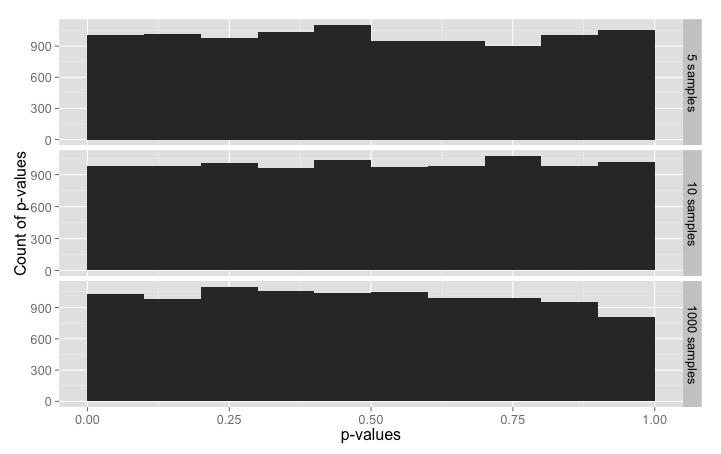
\includegraphics[scale=0.37]{pValueHistPlot.png}
\centering
\end{figure}
Though there are some peaks and valleys the data is fairly even. 
Next are given the code to plot the t distribution against the normal distribution on the same graph::
\begin{verbatim}
> ggplot(NULL, aes(x=x, colour = distribution)) + 
+   stat_function(fun=dnorm, data = data.frame(x = c(-6,6), distribution = factor(1))) + 
+   stat_function(fun=dt, args = list( df = 20), data = data.frame(x = c(-6,6), 
+   distribution = factor(2)), linetype = "dashed") +   scale_colour_manual(values = 
+   c("blue","red"), labels = c("Normal","T-Distribution"))
\end{verbatim}
\begin{figure}[!h]
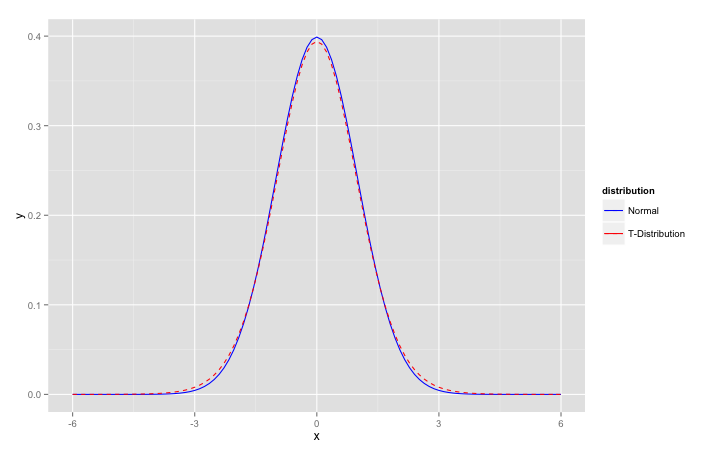
\includegraphics[scale=0.37]{tDistLinePlot.png}
\centering
\end{figure}
Now the same histogram plot we did with the normal distribution is done with the t distribution using the \verb|rt| command to generate random t distribution plot:
\begin{verbatim}
> my.data <- rt(n.rand, df = 20)
> p.df.m <- assign_vector(my.data, n = n.test)
No id variables; using all as measure variables
> ggplot(p.df.m, aes(x = value)) + 
+   geom_histogram(binwidth = 1/10) + 
+   facet_grid(facets=variable ~ ., scales="free_y") + 
+   xlim(0,1) +
+   ylab("Count of p-values") +
+   xlab("p-values") +
+   theme(text = element_text(size = 16))
\end{verbatim}
\begin{figure}[!h]
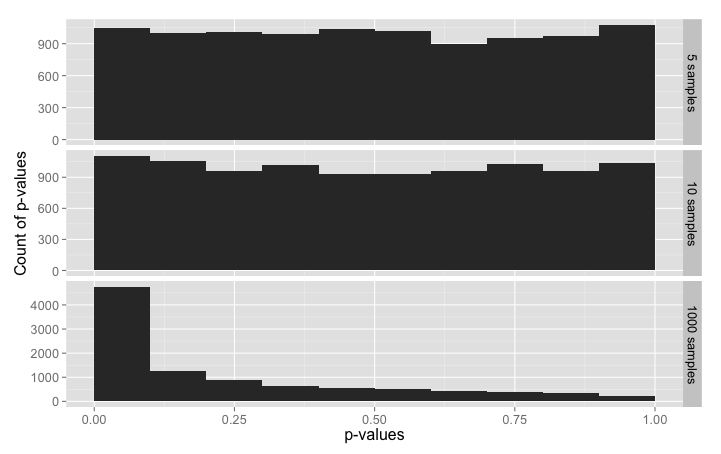
\includegraphics[scale=0.37]{tDistHistPlot.png}
\centering
\end{figure}
Here it shows that at the 1,000 sample level, the t distribution starts to look different than the normal distribution.\\
Next the exercise has us testing the tails of the distribution by removing the tails from the t distribution that are above 3 and below -3 and then replacing them with values from the normal distribution.
\begin{verbatim}
> my.data <- rt(n.rand, df = 20)
> my.data.2 <- rnorm(n.rand)
> my.data <- my.data[which(my.data < 3 & my.data > -3)]
> my.data <- c(my.data, my.data.2[which(my.data.2 < -3 | my.data.2 > 3)])
> p.df.m <- assign_vector(my.data, n = n.test)
No id variables; using all as measure variables
> ggplot(p.df.m, aes(x = value)) + 
+   geom_histogram(binwidth = 1/10) + 
+   facet_grid(facets=variable ~ ., scales="free_y") + 
+   xlim(0,1) +
+   ylab("Count of p-values") +
+   xlab("p-values") +
+   theme(text = element_text(size = 16))
\end{verbatim}
Now the graph looks closer to the Normal histogram which would mean that the tails are affecting these outputs quite a bit. 
\pagebreak
\begin{figure}[!h]
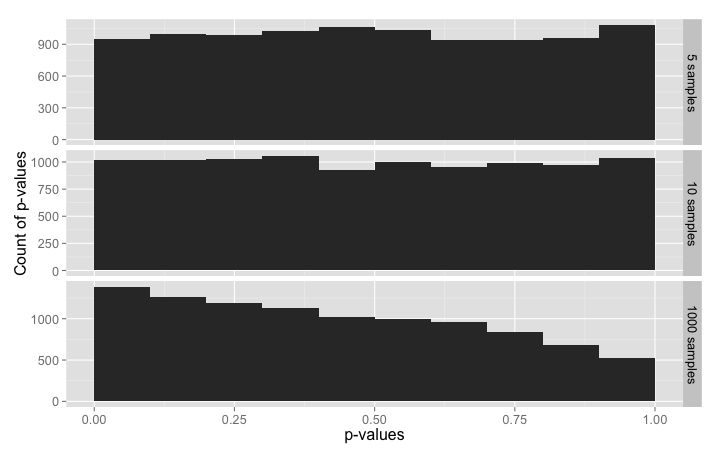
\includegraphics[scale=0.37]{tDistNormalTails.png}
\centering
\end{figure}\\
Next, they have us do the exact opposite:
\begin{verbatim}
> my.data <- rnorm(n.rand)
> my.data.2 <- rt(n.rand, df = 20)
> my.data <- my.data[which(my.data < 3 & my.data > -3)]
> my.data <- c(my.data, my.data.2[which(my.data.2 < -3 | my.data.2 > 3)])
> p.df.m <- assign_vector(my.data, n = n.test)
No id variables; using all as measure variables
> ggplot(p.df.m, aes(x = value)) + 
+   geom_histogram(binwidth = 1/10) + 
+   facet_grid(facets=variable ~ ., scales="free_y") + 
+   xlim(0,1) +
+   ylab("Count of p-values") +
+   xlab("p-values") +
+   theme(text = element_text(size = 16))
\end{verbatim}
\begin{figure}[!h]
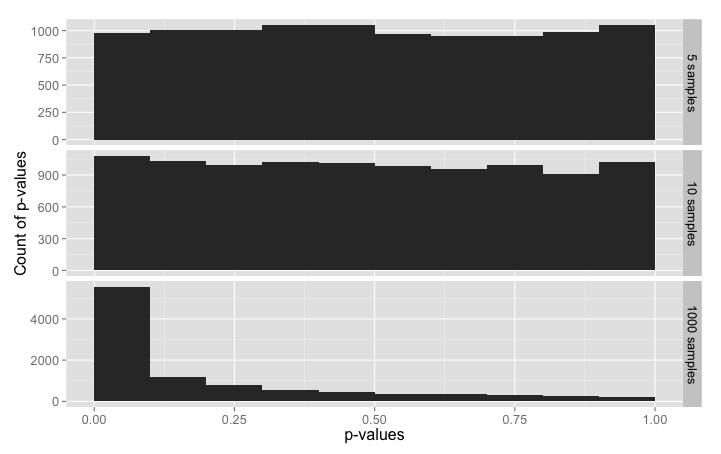
\includegraphics[scale=0.37]{nDistTtails.png}
\centering
\end{figure}
Now the graph looks almost the same as the t distribution graph except that 99\% of the data is coming from the normal distribution.\\
Last the same test is ran on a skewed data set:
\begin{verbatim}
> my.data <- rlnorm(n.rand, 0, 0.4)
> qplot(my.data, geom = "histogram") + xlab("x")
stat_bin: binwidth defaulted to range/30. Use 'binwidth = x' to adjust this.
> p.df.m <- assign_vector(my.data, n = n.test)
No id variables; using all as measure variables
> ggplot(p.df.m, aes(x = value)) + 
+   geom_histogram(binwidth = 1/10) + 
+   facet_grid(facets=variable ~ ., scales="free_y") + 
+   xlim(0,1) +
+   ylab("Count of p-values") +
+   xlab("p-values") +
+   theme(text = element_text(size = 16))
\end{verbatim}
\begin{figure}[!h]
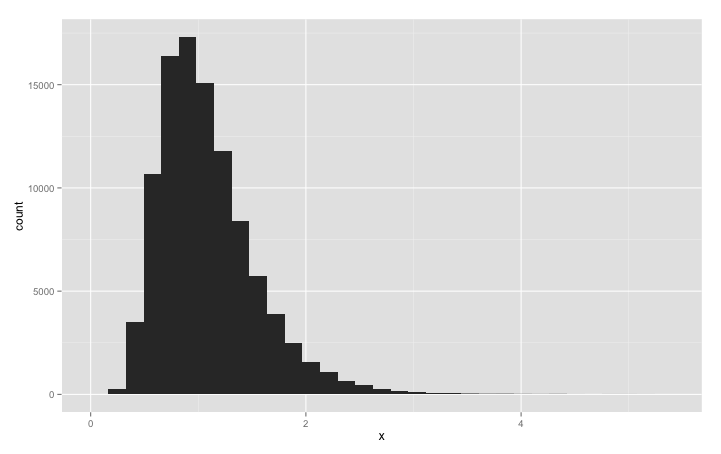
\includegraphics[scale=0.37]{histPlotSkew.png}
\centering
\end{figure}
\begin{figure}[!h]
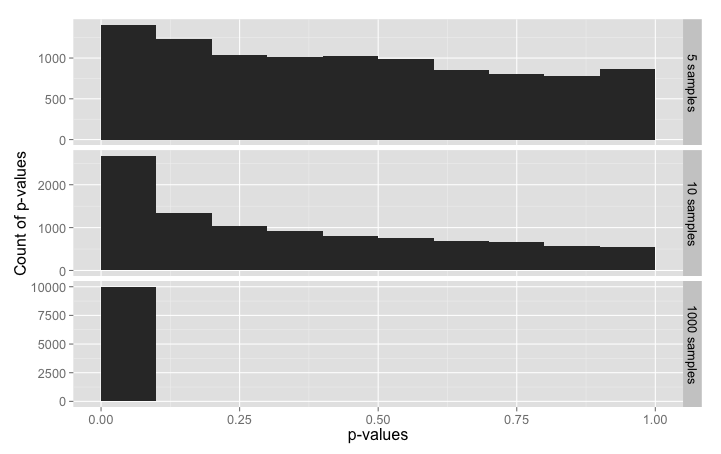
\includegraphics[scale=0.37]{skewHistPlot.png}
\centering
\end{figure}
Again at the small sample size the data set looks normal. The point this exercise is trying to get across is that normality tests can only get you so far that ultimately you need to use judgement to determine if the dataset is normal and use these types of test to catch very large errors. 
\end{document}
